\chapter{Verteilungsalgorithmus}
\label{chapter:algorithm}
    Im folgenden Kapitel wird der Algorithmus zum Verteilen der Studenten anhand der Präferenzlisten auf die Kurse vorgestellt.
    Zunächst wird im ersten Abschnitt eine geeignete Zielfunktion aufgestellt und kurz erklärt.
    Anschließend werden verschiedene Varianten für die Parameter diskutiert.
    Darauffolgend wird auf die Einbindung in das Backend eingegangen.
    
    \section{Aufstellen Zielfunktion}
        Ausgangspunkt für die Zielfunktion des Verteilungsalgorithmus ist eine Matrix $ X \in \{0,1\}^{n \times m}$, wobei $ n $ die Anzahl der Studenten und $ m $ die Anzahl der Kurse ist.
        Ein Eintrag in dieser Matrix $ x_{ij} $ kodiert, ob ein Student einem Kurs zugeordnet wurde, auf folgende Weise:
        wurde ein Student $ i $ dem Kurs $ j $ zugeteilt, dann ist $ x_{ij} = 1 $, wenn nicht, dann gilt $ x_{ij} = 0 $. 
        Diese $ x_{ij} $ sind die Variablen der Zielfunktion.
        Das bedeutet, es wird nach einer Belegung der Einträge $ x_{ij} $ der Matrix $ X $ gesucht, so dass in jeder Zeile der Matrix immer genau ein Eintrag auf $ 1 $ gesetzt ist.
        Das ist gleichbedeutend mit der Aussage, dass jeder Student genau einem Kurs zugeteilt wurde.
        Daraus ergibt sich die Zielfunktion zu
            $$ \max \sum_{i=1}^{n} \sum_{j=1}^{m} c(i,j)x_{ij}  ~~~,$$
        dabei bezeichnet $ c(i,j) $ eine Gewichtsfunktion.
        Die Gewichte bilden die Parameter der Zielfunktion.
        
        Zusätzlich zu dieser linearen Zielfunktion ist es notwendig zwei Nebenbedingungen zu formulieren, um die oben beschriebene Idee der Matrix $ X $ zu formalisieren.
        Zum einen müssen die $ x_{ij} $ nur die Werte $ 0 $ oder $ 1 $ annehmen können:
            $$\forall {i \in \{1,..,n\}} \forall {j \in \{1,..,m\}}:  x_{ij} \in \{0,1\} ~~~.$$
        Zum anderen soll jeder Student nur einem Kurs zugeteilt werden:
            $$ \forall {i \in \{1,..,n\}}: \sum_{j=1}^{m} x_{ij} = 1 ~~~.$$
        
        Zuletzt ist mit einer dritten Nebenbedingung die Teilnehmerzahl für die Kurse zu begrenzen:
             $$ \forall {j \in \{1,..,m\}}: t_{\min}(j) \leq \sum_{i=1}^{n} x_{ij} \leq t_{\max}(j) ~~~,$$
        dabei bezeichnet $ t_{\min}(j) $ die minimale und $ t_{\max}(j) $ die maximale Teilnehmerzahl eines Kurses $ j $.
        
    \section{Erweiterung der Zielfunktion und Wahl der Parameter}
        Die Parameter der Zielfunktion können frei gewählt werden.
        In diesem Abschnitt sollen verschiedene Varianten dargestellt werden, wie die Gewichte gewählt werden können bzw. wie die Zielfunktion weiter angepasst und erweitert werden kann.
        
        \subsection{Lineare Gewichte}
            Die nahe liegende Wahl der Gewichte ist, die Präferenzliste der einzelnen Studenten für die Kurse zu verwenden.
            Da versucht wird, die $ x_{ij} $ so zu wählen, dass die Summe maximal wird, wird so eine Zuordnung eines Studenten zu einem Kurs, für den er eine höhere Präferenz angegeben hat, gegenüber einem mit einer niedrigen Präferenz bevorzugt.
            Der sogenannte \textit{Score} der Funktion, also das Ergebnis der Summe, wird somit höher, je mehr Studenten in von ihnen gewünschte Kurse verteilt werden.
            
        \subsection{Exponentielle Gewichte}
            Eine zweite Variante ist, die Gewichte nicht nach der Präferenzliste, also linear und in gleichen Abständen, zu wählen, sondern exponentiell.
            Dadurch wirkt sich das Zuteilen eines Studenten auf einen Kurs, dem er eine hohe Präferenz gegeben hat, deutlich stärker auf den \textit{Score} aus, als in der vorherigen Variante.
            Oder andersherum: das Zuteilen zu einem Kurs mit niedriger Präferenz wird stärker mit einem niedrigen Score bestraft.\\
            
            In Abbildung \ref{fig:weights} sind die beiden verschiedenen Gewichtungen gegenübergestellt.
            Wie bereits erwähnt, bestraft die exponentielle Gewichtung die Zuteilung zu Kursen mit niedriger Präferenz deutlich stärker als die lineare Gewichtung.
            
            \begin{figure}
                \centering
                \begin{subfigure}{0.49\textwidth}
                    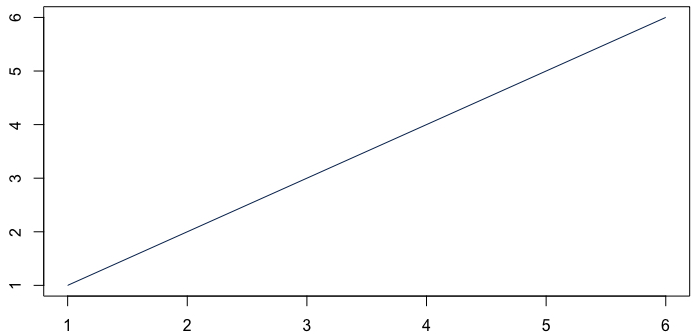
\includegraphics[width=1.0\textwidth]{./algorithm/images/lin_weights.png}
                \end{subfigure}
                \begin{subfigure}{0.49\textwidth}
                    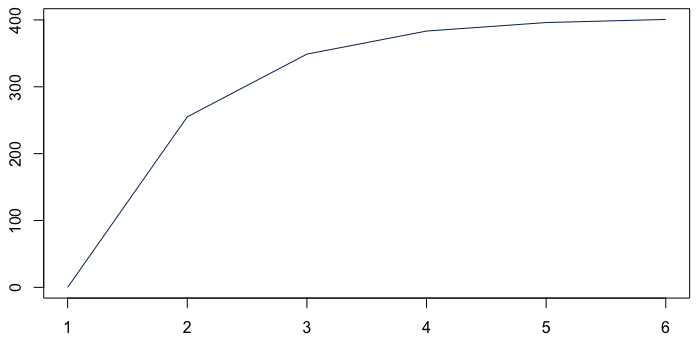
\includegraphics[width=1.0\textwidth]{./algorithm/images/expo_weights.png}
                \end{subfigure}
                \caption{Gegenüberstellung von linearer Gewichtung (links) und exponentieller Gewichtung (rechts). Die horizontale Achse bezeichnet die Präferenzen, die vertikale den Wert des Gewichts}
                \label{fig:weights}
            \end{figure}
            
        
        \subsection{Festes Minimum}
            Die Gewichte können bei dieser Erweiterung der Zielfunktion weiterhin frei gewählt werden. 
            So sind zum Beispiel die beiden Ansätze aus dem vorherigen Abschnitt denkbar.
            Allerdings wird hier zusätzlich ein festes Minimum für die kleinste noch zulässige Präferenz angegeben.
            Das bedeutet, dass kein Student einem Kurs zugeteilt wird, dem er eine geringere Präferenz als das Minimum gegeben hat.
            Dies wird umgesetzt, indem die zweite Nebenbedingungen aufgeteilt wird.
            Jeder Student muss genau einem Kurs mit ausreichender Präferenz zugeteilt werden:
            $$ \forall {i \in \{1,..,n\}}: \sum_{\{j \in \{1, \dots, n\} \mid c(i,j) \geq \text{minPref}\}} x_{ij} = 1 ~~~,$$
            und jeder Student darf keinem Kurs mit zu kleiner Präferenz zugeteilt werden:
            $$ \forall {i \in \{1,..,n\}}: \sum_{\{j \in \{1, \dots, n\} \mid c(i,j) < \text{minPref}\}} x_{ij} = 0 ~~~,$$
            dabei bezeichnet $ \textsf{minPref} $ das entsprechend der Gewichtsfunktion transformierte Minimum.
            
            Das Anwenden dieser Methode hat den Vorteil, dass das Minimum fest gewählt werden kann und somit garantiert ist, dass kein Student schlechter als das Minimum eingeteilt wird.
            Dadurch kann es jedoch dazu kommen, dass einige Studenten in ihrer Präferenz zugunsten des festen Minimums fallen oder auch, dass bei einem zu hohen Minimum keine Lösung für das Problem gefunden werden kann.
            
        
        \subsection{Betrachtung der Varianz}
            Eine weitere Anpassung der Zielfunktion könnte die Erweiterung um einen zusätzlichen Term sein.
            Es ist so denkbar, die Varianz als Maß für die Streuung mit in die Zielfunktion einzubeziehen.
            Formal würde das zu folgender Zielfunktion führen:
                $$ \max \sum_{i=1}^{n} \sum_{j=1}^{m} c(i,j)x_{ij} 
                                ~-~ \frac{\beta}{n} \sum_{i=1}^{n}
                                    \left[\left(\sum_{j=1}^{m} c(i,j)x_{ij}\right) - \frac{1}{n} \sum_{i=1}^{n} \sum_{j=1}^{m} c(i,j)x_{ij}\right]^2 ~~~,$$
            dabei bezeichnet der hintere Term die empirische Varianz. $ \beta $ ist ein weiteres Gewicht, um den Einfluss der Varianz zu steuern.
            Mithilfe dieser Zielfunktion wird nun nicht nur versucht jeden Studenten in einen für ihn möglichst guten Kurs zuzuteilen, sondern auch die Varianz zu minimieren.
            Damit werden nach Möglichkeit alle Studenten in einen ähnlich von ihnen präferierten Kurs verteilt, oder mit anderen Worten, es werden Ausreißer verhindert.\\
            
            Nachteil bei dieser Variante ist jedoch, dass die Zielfunktion nun nicht mehr linear, sondern quadratisch ist.
            Zum einen erhöht das den Aufwand, um eine Lösung zu finden, enorm.
            Zum anderen kann mit bekannten Algorithmen zum Lösen solch quadratischer Probleme das Finden einer optimalen Lösung nicht garantiert werden.
            Aus diesem Grund wurde bei der Umsetzung des Verteilungsalgorithmus die zuvor gezeigte lineare Zielfunktion verwendet.
           
            
        